%% ----------------------------------------------------------------
%% Progress.tex
%% ---------------------------------------------------------------- 
\documentclass{ecsreport}  
\usepackage{libertine}
\usepackage{rotating}
\usepackage[ngerman,english]{babel} % Use the progress Style
\newcommand{\code}[1]{\texttt{#1}}
\usepackage[backend=biber, style=authoryear]{biblatex}  % Location of your graphics files
\addbibresource{Bibliography.bib}
\usepackage{tabu}
\usepackage{float}
\hypersetup{colorlinks=true}   % Set to false for black/white printing
%
\definecolor{purple}{rgb}{0.65, 0.12, 0.82}
\lstset{
	breakatwhitespace=true,
	breaklines=true,
	keywordstyle=\color{blue}\bfseries,
	identifierstyle=\color{black},
	commentstyle=\color{purple}\itshape,
	stringstyle=\color{red},
	float=here
}

\lstdefinelanguage{javascript}{
	keywords={break, case, catch, continue, debugger, default, delete, do, else, false, finally, for, function, if, in, instanceof, new, null, return, switch, this, throw, true, try, typeof, var, void, while, with},
	morecomment=[l]{//},
	morecomment=[s]{/*}{*/},
	morestring=[b]',
	morestring=[b]",
	ndkeywords={class, export, boolean, throw, implements, import, this},
	sensitive=true
}            % Include your abbreviations
%% ----------------------------------------------------------------
\begin{document}
\frontmatter
\title      {A Gloss and Difficulty Rating System to Assist with the Discovery and Reading of German Language Articles}
\authors    {\texorpdfstring
             {\href{mailto:stp1g15@ecs.soton.ac.uk}{Steffan T. Padel}}
             {Steffan T. Padel}
            }
\addresses  {\groupname\\\deptname\\\univname}
\date       {\today}
\subject    {}
\keywords   {}
\supervisor {Prof. Adam Prugel-Bennett}
\examiner   {Prof. Lie-Liang Yang}
\maketitle
\begin{abstract}
	
This report proposes and then details the development and testing process of a gloss application designed to help German language learners discover and then read authentic articles from German news sources. It begins by outlining the application before starting research into the logic and methods such an application would use. Once these have been decided on, the project then goes on to detail how the application was designed and programmed, listing the choices made and the reasoning behind them. The report then details and analyses the results of user testing on the application, before performing a critical evaluation of the both the application and the project as a whole, detailing their flaws and the various methods by which they could be improved. The report then concludes by examining how the application could be improved for a future commercial version before deciding that such improvements are not viable.	 
	
\end{abstract}
\tableofcontents
\listoffigures
\listoftables
\lstlistoflistings
\mainmatter
%% ----------------------------------------------------------------
\chapter{Introduction}

\section{Problem}
While learning a second language, many learners encounter problems while trying to find and read texts written in the language they are learning. Modern technology has helped with this to some regard, with development of glosses, which are digital tools that provide prompts for vocabulary words. These prompts can be translations of the words, definitions in the source language, audio visual materials or any combination of the above. 

The problem most glosses developed today have is that they are specifically tailored for the text they are being used on. The words that can be examined are pre-selected, the gloss content is pre-written and the text has been pre-selected. This still leaves multiple problems for the user: They could not find the text interesting, they could already know the words in the gloss or they might find the text too easy. 

\section{Solution and Goals}

The solution to this problem was, perhaps unsurprisingly, to develop a prototype application. This application should be able to:

\begin{itemize}
	\item Allow the user to a select a category of articles that they find interesting.
	
	\item Find and pull articles in that category from a variety of news sources.
	
	\item Rate the articles based on their perceived difficulty for the user.
	
	\item Allow the user to activate a gloss on any and all words in the article. 
\end{itemize}

To make sure as many platforms are supported as easily as possible, the application will run in a web browser and be hosted remotely. The initial prototype of the application will support German in order to minimise the number of variable that need to be taken into account and because German is a language the developer can speak, allowing for easier development of the application.

Once developed, this  prototype application will then be user tested by a number of German learners of varying experience levels. They will provide feedback on their experiences using the application, which will then be examine and used to formulate the idea of a release build.          % Proofreading 1
\chapter{Application Development Plan}

A visualization for the plan for this project can be seen in the Gannt chart in figure \ref{fig:gannt}
\begin{figure}
	\caption[Gannt Chart of the Project]{Gannt chart showing the project's planned process over the academic year.}
	\label{fig:gannt}
	\begin{center}
	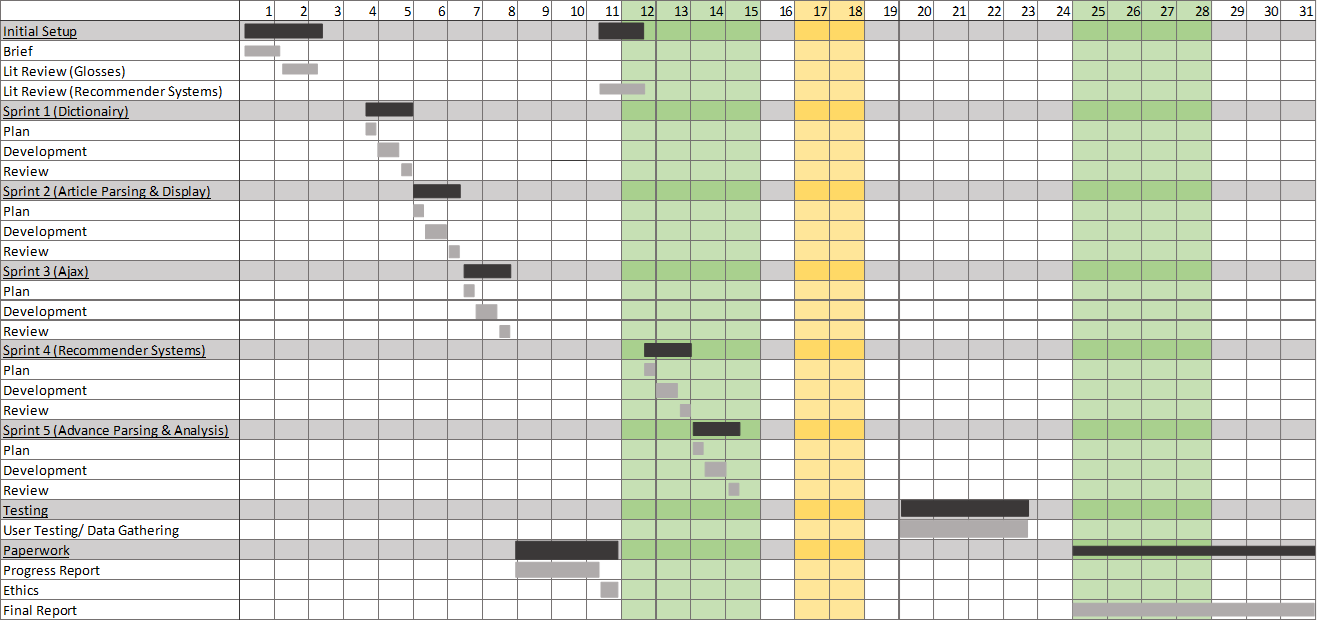
\includegraphics[width=\textwidth]{Graphics/Gannt}
	\end{center}
\end{figure} 

\section{Readings and Research}

The plan details that reading was to be divided into two parts, reading about glosses and reading about difficulty rating systems. With the reading about difficulty rating systems being done after the gloss was developed. This was done as the difficulty rating system was not part of the minimum viable project, so the reading about it could be left until after the development of the minimum viable project was complete. The vast majority of this reading was academic, looking into the effectiveness of various glosses and methods of rating the difficulty of articles.

Other reading was done during the planning stage of each sprint, this reading was more technical and was about researching and deciding upon the technologies that were to be used for that sprint. Once a technology had been decided upon, there was some time spent on learning how to integrate it with project.


\section{Development}

The application was developed using AGILE methods. these methods were used as they allowed the developer to have regular meetings with the project supervisor, discussing the progress made, what was left to be done whether or not it was achievable.

\section{Testing}

Three types of testing were done on the application. Unit testing was during the development of sprint one, to ensure that the application was interacting with the dictionary API correctly, making sure that the correct translations of various words were found. 

functional testing was during the development of the rest of the application, the developer would use the application, testing whether or not the feature they were currently implementing was working as planned.

Finally, user testing was done once all six sprints were completed, it consisted on the user using the application to read three articles, and then filling out a feed back survey about their experiences with it. In addition, the user's use of the application was tracked, seeing what words they requested and what articles they read. Ethics approval for this test was obtained from the ECS ethics board.           % Proofreading 1
\chapter{Background Reading}

Reading for the project can be divided into reading about the gloss aspect of the application, and then reading about a difficulty rating system. Each of these parts of the reading happened independently, as their subject matter are largely unrelated.


\section{Glosses}

The research done into glosses is divided into to parts, the first being research into whether or not glosses are effective, the second part was about the various designs of glosses, trying to discover which ones were the most effective.

\subsection{Effectiveness of Electronic Glosses}

\textcite{abraham2008} finds that, overall, that learners with access to an electronic gloss will perform better than learners without access, in both skills of reading comprehension and vocabulary retention, particularly on intermediate learners. They note that the small sample size of studies analysed should mean that their study is not seen as conclusive evidence, however suggestive evidence is enough to establish that development of this project should continue.

Another caveat that should also be added that most of the studies analysed in \textcite{abraham2008} are of tailor-made glosses designed for a specific text, as such the research findings of these studies and the meta-study may not be fully applicable to this project.


\subsection{Design Methods of Electronic Glosses}

\textcite{roby1999} identifies three main parts of a gloss' design, its presentation, its taxonomy and its density. However, as density, which is the amount of content in the gloss, is something determined by the user, background reading into design was limited to presentation and taxonomy. 

\subsubsection{Gloss Presentation}

Gloss presentations is how the gloss is presented relative to the text. 

\textcite{chen2016} identifies the three most researched gloss presentations as: in-text, marginal and pop up.  \textcite{abuseileek2008} finds that out of these three the marginal presentation category performs the best in both vocabulary retention and reading comprehension, while \textcite{marefat2016} finds that pop-ups are more effective than marginal for reading comprehension. As \textcite{chen2016} says, there has not been sufficient research into gloss location for valid conclusions to be drawn. 

\subsubsection{Gloss Taxonomy}

Gloss taxonomy is the content of the gloss.

\textcite{gettys2001} finds that dictionary style translations perform better than sentence level translations, suggesting that it would be better to translate the dictionary form of the word, providing information about how the word changed from its dictionary form to its current form in the article. 

There is a large body of research that suggests that providing multimedia glosses is more effective than providing text only ones. \autocite{yoshii2006, kost1999}. This is harder to implement  as it would the application to have a better understanding of the word's context to provided an accurate image of the word. 


\section{Article Difficulty Rating}

The reading for this section of the application was harder to find, little has been written about the discovery and difficulty rating of texts for second language learners in general, or German learners in specific. 

The easiest method of calculating the difficulty of an article seems to be a mathematical expression of it's readability, called a readability index. Perhaps the most famous of these being the Flesch Reading Ease (FRE) formula \autocite{flesch1948}. This formula is for America English, however similar formulae have been developed for German, two of these are highlighted below.

The first formula for German is an adaptation of the FRE formula as proposed in \textcite{amstad1978}, this relies on much the same model as the original FRE formula, however takes into account the longer average word length in the German language, this formula is show in figure \ref{fig:fre} where  ASL is the average sentence length and ASW is the average syllables per word. This formula maps the readability of the text onto a range of 0 to 100, with 0 being easy and 100 being hard. 

\begin{figure}[H]
	\caption[Flesch Reading Ease Formula]{Formula for the German adaptation of the Flesch reading ease formula, a method of calculating the readability of a German language text}
	\label{fig:fre}
	\begin{center}
		\begin{math}
		FRE = 180 - ASL - 58.5 \times ASW
		\end{math}
	\end{center}
\end{figure}

The other readability index for German is the  Wiener Sachtextformel (WSTF) as proposed in \textcite{bamberger1984}, on version of this is as shown in figure \ref{fig:wst}. Where MS is the percentage of words with three or syllables, SL is the average sentence length, IW is the percentage of words with six or more characters and ES is the percentage of monosyllabic words. This formula maps the difficulty rating onto a range of 4 to 15, with the lower numbers being easier. This is done to reflect the German school year that is believed to be appropriate for that level of text.

\begin{figure}
	\caption[Erste Wiener Sachtextformel Formula]{The Erste Wiener Sachtextformel formula, one method of calculating the readability of German language texts. }
	\label{fig:wst}
	\begin{center}
		\begin{math}
		WSTF = 0.1935 \times MS + 0.1672 \times SL + 0.1297 \times IW - 0.0327 \times ES - 0.875
		\end{math}
	\end{center}
\end{figure}

The two formulas are commonly used together when assessing the readability of texts, being used in a variety of studies, such as \textcite{rottensteiner2010} which uses them both to assess the readability of newly published textbooks. This publication also notes that these formulae only measure the linguistic complexity of the article, ignoring other factors, such as presentation, that influence how easy the article is to read. 

In addition to the formulae listed above there are methods of determining a readability ranking through the use of machine learning. \textcite{hancke2012} which attempts to build a readability classification system from a corpus of articles. This paper looks a lot more in depth at a lot of features of the text. However, this model only performed 7.5\% better than the computational scores calculated from the traditional formula. Given the time constraints and the already complex nature of the project, it would not be worth the effort to implement such a model, as the tradition formulae such as WSTF and FRE perform well enough for the purposes of this project.     % Proofreading 1
\chapter{Proposed Application}

Below is a rough outline of the application and list of the development sprints for the application. More detailed descriptions of both the design of the application and the server side logic of the application are presented in later chapters. 

\section{Outline}

The outline of the application is as follows: 

The user starts the application by selecting a category of articles and their level of experience with German. From there, they are presented with a list of articles in that category, with each article having a difficulty rating. The user can then select an article based on the title of the article as well as the difficulty rating.

Once the user has selected the article, they are presented with the text of the article. From here, they can click on words in the article, and the application will show them a translation of the word and grammatical information about the word in a marginal gloss form. These gloss element can then be removed from the screen when no longer needed.

A marginal gloss was chosen as one of those is easier to implement than the other gloss presentation methods, while the decision to use dictionary level translations was made as they are effective and easier to implement than a more effective multimedia gloss.

A systems flow diagram of the basic outline of the application can be seen Figure \ref{fig:sf}

\begin{figure}
	\caption{Wireframe Mockup of the Category Input View}
	\label{fig:sf}
	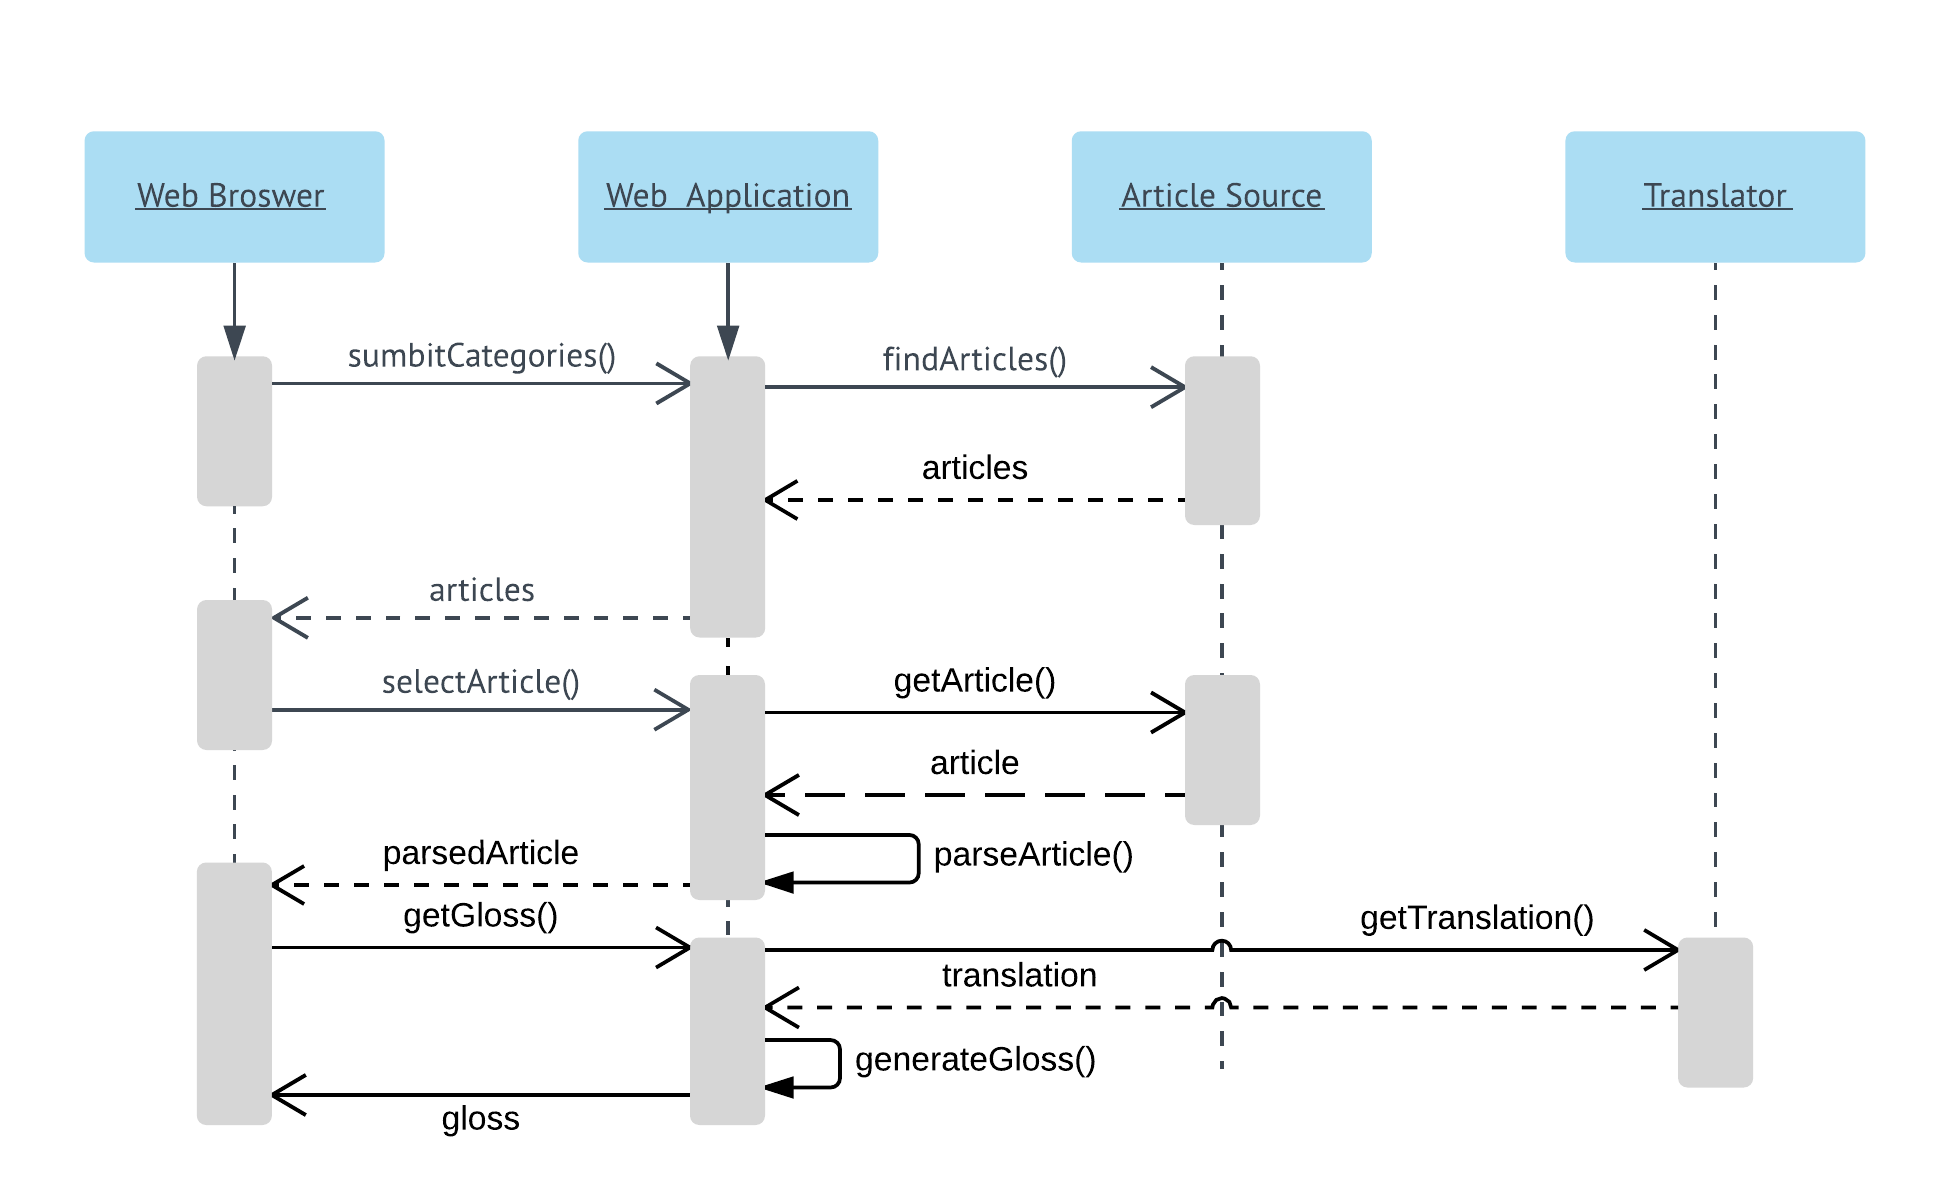
\includegraphics[width=\textwidth]{Graphics/SystemsFlow}
\end{figure}

\section{Development}

Development of the application was divided into six sprints and they were completed in the order in which they are described. The order was chosen as it would allow the application to reach minimal viable project status as soon as possible (end of Sprint 3), leaving the more advanced sprints for later. The sprints are detailed below.

\begin{enumerate}
	\item \textbf{Translation Lookup}
	
	The aim of this sprint is to establish a valid method to retrieve single word translation and grammatical data.
	
	\item \textbf{Article Parsing \& Presentation}
	
	The aim of this sprint is develop a method for the parsing of articles and then to present them through a web browser
	
	\item \textbf{AJAX}
	
	The aim of this sprint is to develop the JavaScript code that will allow the gloss to display entries.
	
	\item \textbf{Advance Parsing}
	
	The aim of this sprint is to allow advanced parsing methods to be performed on the text. Allowing for parts of speech identification of words. 
	
	\item \textbf{Article Discovery}
	
	The aim of this sprint is get the application to find articles on it's own, removing the need for the user to find their own articles.
	
	\item \textbf{Difficulty Rating System}
	
	The aim of this sprint it to develop the system that allows the application to rate how difficult the user will find various articles. 
	
\end{enumerate}
   % Proofreading 1
\chapter{Application Design}

This chapter details the user interface and design elements of the application, specifically how the application appeared when the user testing took place. It details the design decisions made and then proceeds to explain and justify why it was thought that making these decisions would improve the user experience.

\section{Category and Experience Selection}

When the user first connects to the web application, they are shown the view in Figure \ref{fig:view1}. This view allows them to input their experience with German, as well as selecting the category of article that they wish to read. Four different experience levels are available, "beginner", "intermediate", "advanced" and "near fluent". The decision to categorize language experience this was made as these different experience levels are in English and are commonly used as descriptions of language proficiency. While it would have been possible to use much more formal definitions of language proficiency, for example the Common European Framework of Reference for Language (CEFRL), these definition are not commonly taught and would most likely confuse a large proportion of users. Once "beginner", "intermediate" and "advanced" had been decided upon, the decision was made to add a forth level "near fluent" to distinguish between users who needed barely any help and users who needed some help. It was also believed that fluent German speakers would have no need to use the application, and therefore did not need to be considered when selecting these levels.

\begin{figure}
	\caption[Screenshot of the Category Selection View]{Screenshot of the category selection view, where the user inputs the category of article they want to read, as well as their experience level.}
	\label{fig:view1}
	\begin{center}
	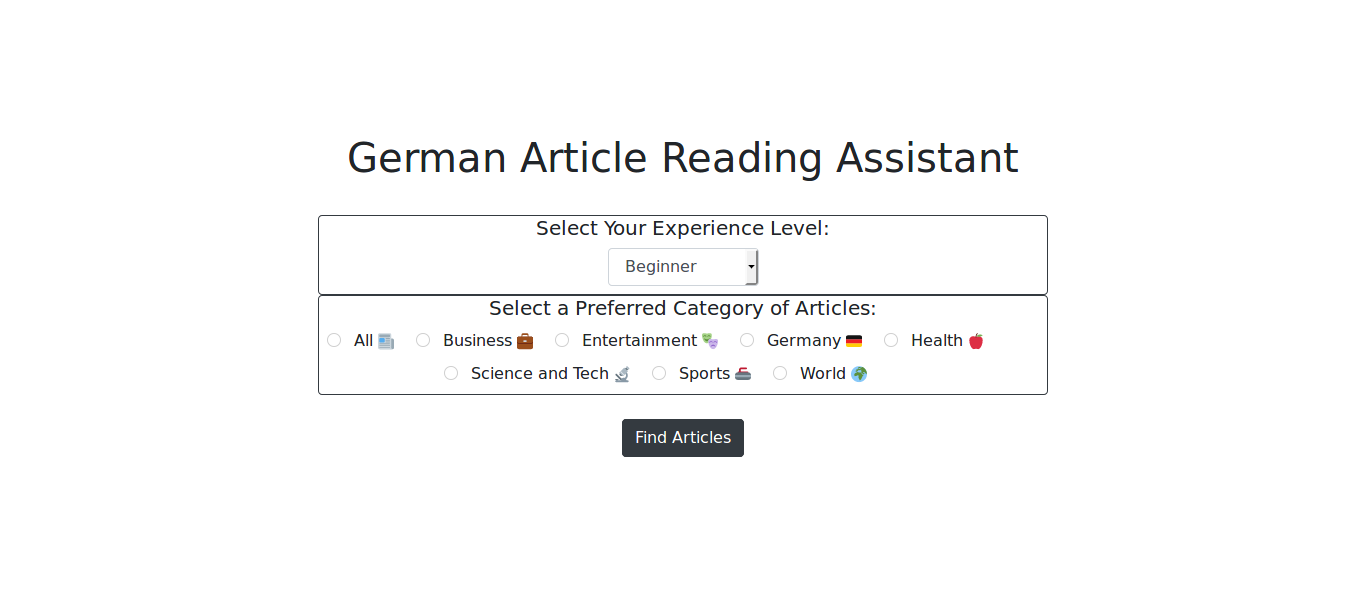
\includegraphics[width=\textwidth]{Graphics/View1}
	\end{center}
\end{figure}

The user then goes on to select a category of article. The selections available are "All", "Business", "Entertainment", "Germany", "Health", "Science and Tech", "Sports" and "World". These categories were chosen to reflect traditional news categories that one would find on a news website. The application originally used German titles for the categories, but they were switched to English as it was believed that some users would not be skilled enough in German to understand the meaning of the titles without access to translations, which are not currently available on this screen. 

An emoji was added next to the name for each category, primarily to make it easier to identify the categories upon sight, but also to broaden the colour pallet being used in the application.

The initial prototype of the application had a different article selection screen, Where the URL of the desired article was inputted instead of a category selection screen. This had both advantages and disadvantages over the current selection model in the final application. This allowed the user to find articles that interested them and then input them into the application and continue reading there, but it also relied on the user having the ability  to find article that interested them externally. Ideally, it would have been best to have both the category selection and direct article input methods implemented with different input screens.

\section{Article Selection}

Once the user has inputted their ability level and desired category of article, they are then presented with the view shown in Figure \ref{fig:view2}. This is a list of articles in the selected category, with titles in German, followed by a difficulty rating. Titles are left in the original German as the user can determine any words that that they do not know from context, making it easier than the categories names to determine. If the user cannot figure out the title, the difficulty ratings provide a clear indication of the level of the articles, suggesting which ones would be suitable for them. 

\begin{figure}
	\caption[Screenshot of the Article Selection View]{An example of the article selection view, here the user is shown a list of articles in their selected category as well as the difficulty rating for each article. They then go on to select an article from the list.}
	\label{fig:view2}
	\begin{center}
	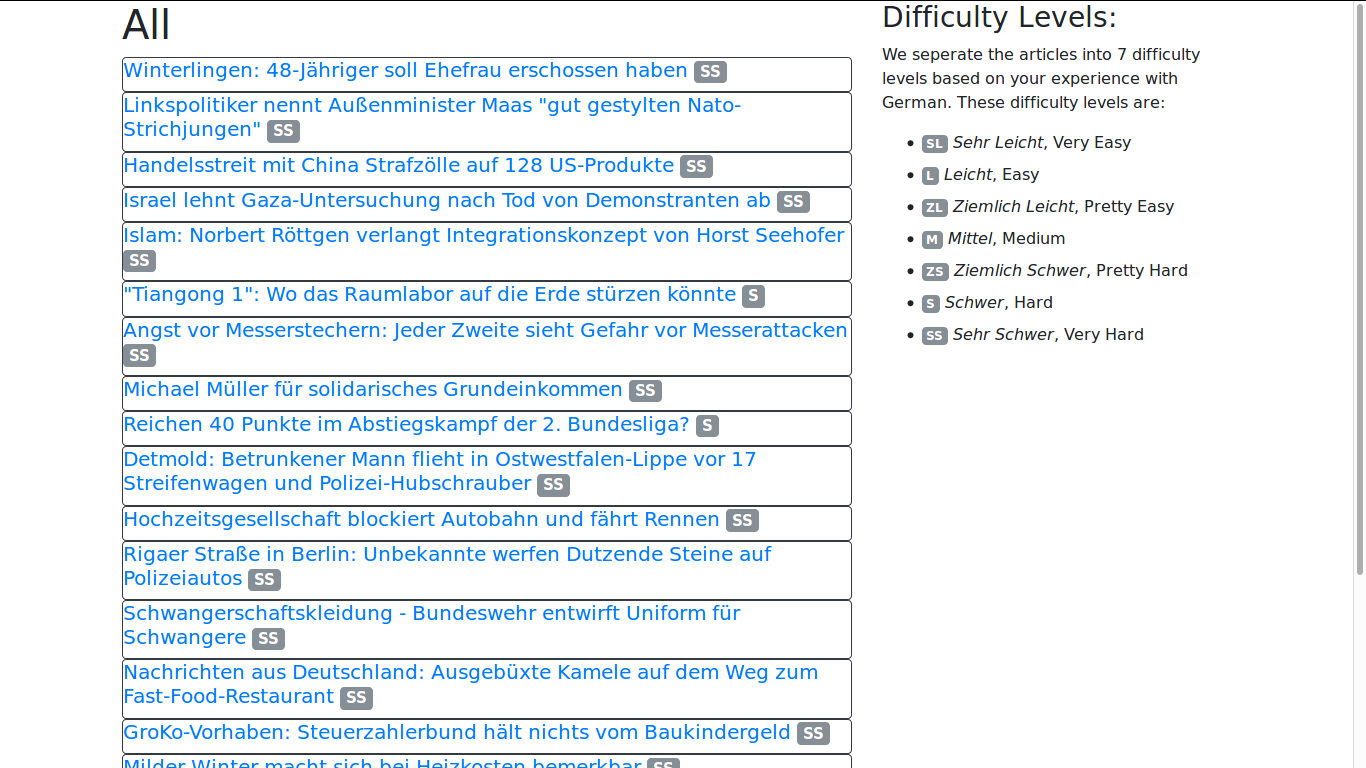
\includegraphics[width=\textwidth]{Graphics/View2}
\end{center}
\end{figure}

To the right of the list of articles, in the position where the gloss will be in the article view, a list of definitions of the different difficulty rating can be seen. These, going in order from most difficult to least are "SS", "S", "ZS", "M", "ZL", "L" and "SL". These difficulty ratings were chosen as they are acronyms of German phrases that translate to the appropriate difficult levels, each one of them having a unique acronym. Seven categories were used, expanding the standard "Easy", "Medium" and "Hard" to include "Very Hard", "Somewhat Hard", "Somewhat Easy" and "Very Easy". These categories can be placed easily on a scale by a user, and then be used to identify with a fair amount  of precision how hard said user will find the article.

The decision to include the definition box was made to make sure that the user could map the German acronyms to corresponding difficulty rating as no full words are used in the rating labels and, as the acronyms come from German words, some users might not be able to deduce the meanings.  

\section{Article Reading}

Once the user has selected an article from the list, they are shown are the view in Figure \ref{fig:view3} which is primarily the content of the article. A button to take the user back to list view is shown to left of the article. On the right of the article text, there is a box which prompts the user to click on words. An additional visual prompt is provided, the cursor changes to the common "pointer" cursor when it is over a word in the article, suggesting that the word can be clicked on.

\begin{figure}
	\caption[Screenshot of the Article Reading View]{The article reading view, where the user can read the contents of their selected article. To the left of the article content is a button taking them back to article selection view and to the right is the gloss column, which contains a prompt telling the user click on articles. }
	\label{fig:view3}
	\begin{center}
	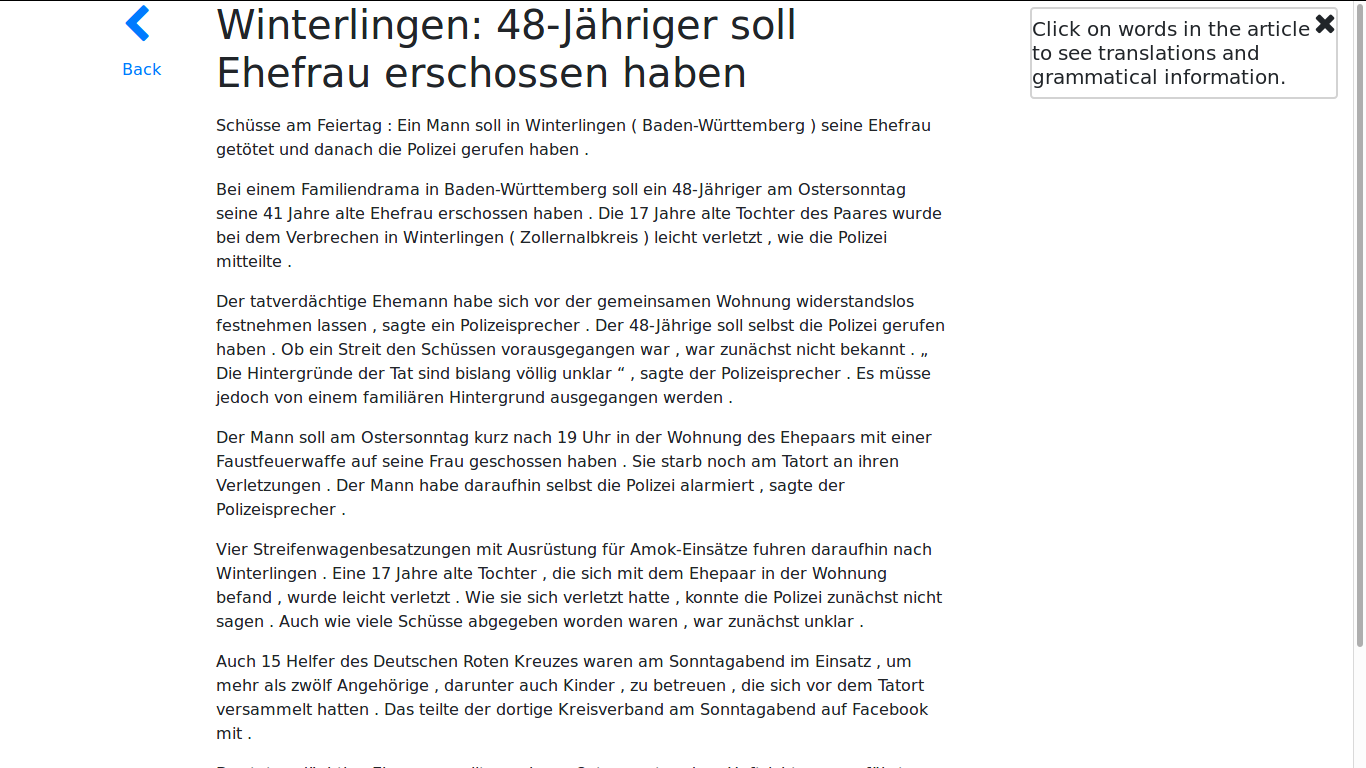
\includegraphics[width=0.7\textwidth]{Graphics/View3}
\end{center}
\end{figure}

Clicking on a word on the article, will make a gloss item appear on the right of the screen, making the screen appear similar to the view shown in Figure \ref{fig:view4}. This positioning makes it marginal gloss, which was found to be effective by \autocite{abuseileek2008}. New items appear at the bottom of the margin and will stay in the margin until they are dismissed by the user. If there are too many gloss entries for the screen, then a scroll bar will appear allowing the user to scroll through the gloss entries independent of that user's scrolling through the article content. The gloss entries are permanent until dismissed as this prevents the user from having to lookup the same word multiple times.

\begin{figure}
	\caption[Screenshot of the Article Reading View with Gloss]{Another screenshot of the article reading view, this time with a gloss entry in the margin.}
	\label{fig:view4}
	\begin{center}
	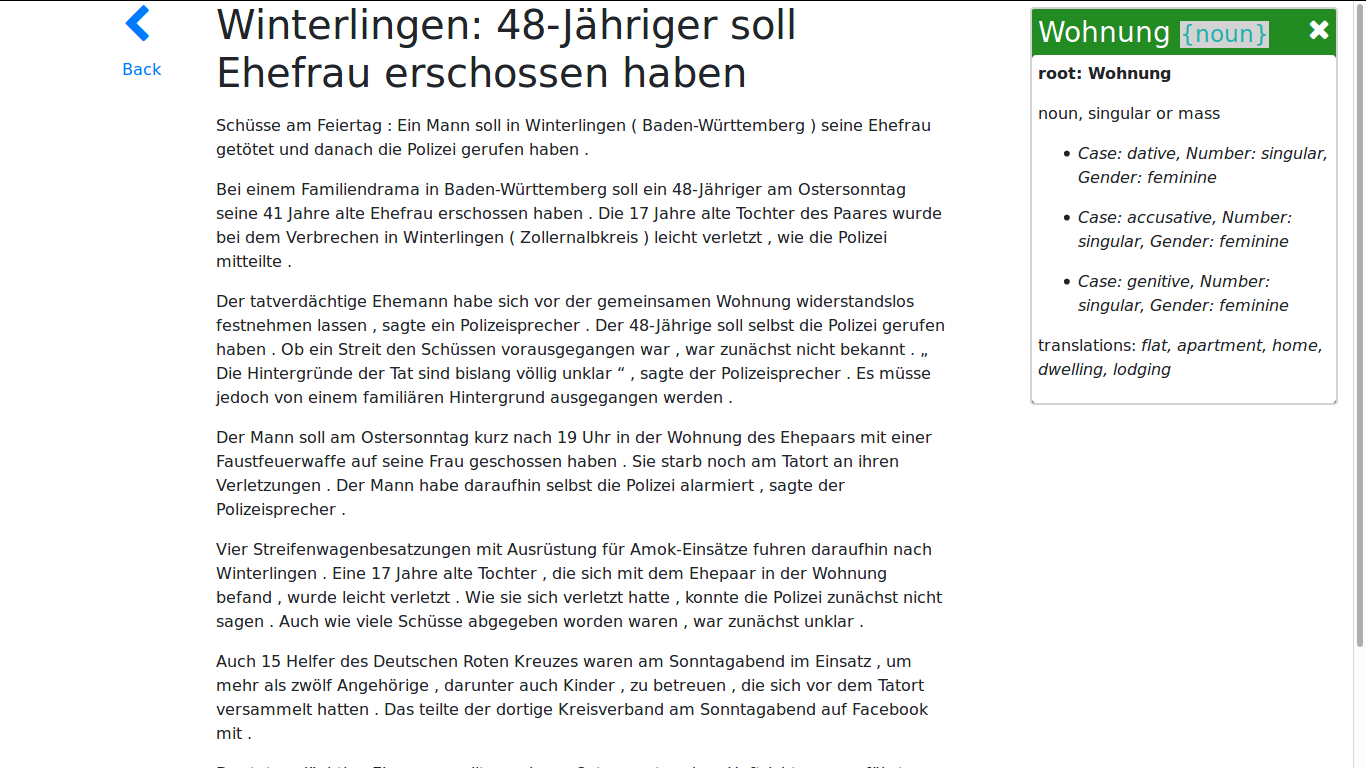
\includegraphics[width=\textwidth]{Graphics/View4}
\end{center}
\end{figure}
 
\subsection{Gloss Items}

\begin{figure}
	\caption{Screenshot of a Gloss Entry}
	\label{fig:gloss}
	\begin{center}
	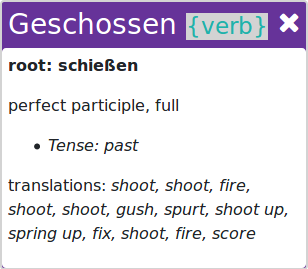
\includegraphics[width=0.3\textwidth]{Graphics/Gloss}
\end{center}
\end{figure}

The design of the gloss items was inspired by a standard dictionary entry. An example of this design can be seen in Figure \ref{fig:gloss}. The top of the gloss is a colour specified by the lexical category of the word; green for nouns, purple for verbs, blue for adjectives, red for any other and black for ones that cannot be identified. The header then contains the form of the words as it appears in the text, followed by the lexical category, in curly brackets, with unique text and background colours. A white cross is on the right of the header, clicking it dismisses the gloss entry, removing it from the gloss. 

The body of the gloss is divided into three parts. The root word, the grammatical information and then possible translations of the root. The root is presented at the top, in bold. This is done so that if the user can identify the word by the root, then they only need to read that. 

After the root, the grammatical information of the word. First is a short description of the word's lexical category and form of the word. Following this is a bullet point list of the possible use cases of the word in this form; Its tense and person if it's a verb, gender, plurality, and case if it's a noun and other relevant information for other lexical categories. 

Finally the body is concluded with various translations of the root words. In the case that the application cannot find a translation, the phrase "no translations found" is presented instead. 
     % Proofreading 1
%TC:envir lstlisting [] xall
\chapter{Application Implementation}

\section{General Technologies and Frameworks}

As it is a web application, HTML, CSS and JavaScript were used for the client side of the application, although this was augmented with both \textit{JQuery} and \textit{Bootstrap} to ease the development of the Javascript and the CSS respectively. 

For the server side of the application, the code was written in python, using the \textit{Flask} framework and its integrated technologies. \textit{Flask} was used as it is easier to user then the alternative python frameworks and the developer has experience using it. python was also chosen for similar reasons and due to the fact that the developer likes it. The memory usage and speed of the various possible programming languages and frameworks was not considered. Ease of use and familiarity were the primary considerations. 

\section{Article Discovery}

For the article discovery portion of the application, the need was for a list of articles, from a variety of sources about a variety of topics. The solution that was found after some search on the internet, was \textit{Google News}.

\textit{Google News} provides several lists of recent articles from different sources divided in different topics, additionally, each of these lists is provided in an RSS feed XML file, a format that allows the code to be written for both URL and title extraction with minimal effort, both on the parts of the developer and the machine life time.

The categories provided by the \textit{Google News} RSS feeds were usable, but overall they were fairly common news categories. On the plus side, these categories are recognisable, on the down side, these categories are not customisable, however, the categories were pre-selected, saving time on artificial category creation, the end user can just selected one of them. The code for obtaining the articles is shown in listing \ref{lst:disc}

\begin{lstlisting}[caption={[Article Discovery Code] Python code for obtaining news articles from the \textit{Google News} RSS feeds.}, label=lst:disc, language=python, float]
    # get the articles in a category
    def lookup(self, category, user_level):

        # get the rss feed
        r = requests.get(CAT_MAP[category]['url'])
        root = ElementTree.fromstring(r.text)

        # get the old articles from memory
        old_aritcles = [a.id for a in self.articles[category]]

        # iterate through the article in the rss feed, extracting the articles
        for item in root.iter('item'):
            url = item.find('link').text
            title = item.find('title').text
            aid = str(uuid.uuid5(uuid.NAMESPACE_URL, url))

            # if the article is not already saved, try to parse and rate it (some articles fail)
            if aid not in old_aritcles:
                try:
                    self.articles[category].append(Article(url, title, aid, category))
                except ZeroDivisionError:
                    print('Zero Divison Error')
                except ArticleException:
                    print('Article Exception')

        # return the list of articles classified.
        return self.classify(self.articles[category], user_level)
\end{lstlisting}


This code takes the category, and then gets the current state of the corresponding RSS feed. It then iterates through item tags in the RSS feed, extracting the title and URL of each tag. It then attempts to parse and rate the article for listing. Once every article has be parsed and rated, it returns a list for display. In addition, articles are stored and added to future lists so that the code doesn't have to reparse an article every time the list is generated.

There were alternatives to the \textit{Google News} RSS feeds that were examined, primarily \textit{NewsAPI}. However this was found to be lacking for two reasons. Primarily, this API would list content, where the primary means of communication was not text. Comics and other image based got added to the lists being provided by the API. As the parser and the gloss system relied on the content being text based and there was no easy way to distinguish being text based content and image based content. The other more minor reason that \textit{NewsAPI} was disregarded was because it was more difficult to categorise the articles, whereas the \textit{Google News} RSS feeds provided pre-created categories, to save time on both filtering out image-based content and the categorisation of articles, the decision was made to use the \textit{Google News} RSS feeds. 


\section{Article Difficulty Rating}

The difficulty rating of the article is calculated using two things, the article text as well as the user's experience level. The user's experience level is obtained from the form the user submitted at the start, while the article text needs to be extracted from the article web page and then analysed.

To extract and then analyse the article, two technologies are used. The first is an article scraping python library called \textit{Newspaper}, the purpose of it is to extract the raw article text from the article web page, making the analysis of it easier. Analysis of the article text is then done through another python library called \textit{SpaCy}, which is a parts-of-speech tagging library, while and add on for it, called \textit{Textacy} provides advanced features such as syllable counting. \textit{SpaCy} provides two  sets of parts of speech tags with different levels of precision. 

Once the article text has been extracted and analysed, it's readability index needs to be calculated, this is done using the Erste Wiener Sachetextformel as described in \textcite{bamberger1984}. The WSTF formula was chosen over the FRE formula because the WSTF formula has a smaller output range. This smaller output range allowed for two things the first was easier mapping onto the user experience level as well as a better understanding of the approximate level of each individual number, as those number correspond directly with the German school years. 

Once the readability score is calculated, it needs to be mapped, using the user experience level onto the difficulty ratings, a simple linear map was chosen for this, the mapping system can be seen in table \ref{tbl:ratings}.

\begin{table}
\centering
\caption{Comparison of Translation Software}
\label{tbl:ratings}
\begin{tabu} to \textwidth{|l|c|c|c|c|c|c|c|}
\hline
\textbf{Rating} & \textbf{SL}      & \textbf{L}       & \textbf{ZL}   & \textbf{M}    & \textbf{ZS}   & \textbf{S}  & \textbf{SS}   \\ \hline
Beginner                  & $ r < 2 $ & $ 2 \leq r < 3 $ & $ 3 \leq r < 4 $ & $ 4 \leq r < 5 $ & $ 5 \leq r < 6 $  & $ 6 \leq r < 7 $ & $ 7 \leq r $    \\ \hline
Intermediate              & $ r < 4 $ & $ 4 \leq r < 5 $ & $ 5 \leq r < 6 $ & $ 6 \leq r < 7 $ & $ 7 \leq r < 8 $  & $ 8 \leq r < 9 $ & $ 9 \leq r $    \\ \hline
Advanced                  & $ r < 6 $ & $ 6 \leq r < 7 $ & $ 7 \leq r < 8 $ & $ 8 \leq r < 9 $ & $ 9 \leq r < 10 $  & $ 10 \leq r < 11 $ & $ 11 \leq r $    \\ \hline
Near Fluent             & $ r < 8 $ & $ 8 \leq r < 9 $ & $ 9 \leq r < 10 $ & $ 10 \leq r < 11 $ & $ 11 \leq r < 12 $  & $ 12 \leq r < 13 $ & $ 13 \leq r $    \\ \hline
\end{tabu}
\end{table}

The primary idea behind these ratings was that a user who was less experienced with German would find have a lower threshold for articles that they find difficult. To do this it was decided that near fluent user would be able to read with some confidence articles with a WSTF score of 10 which corresponds to a native speaker who is 15/16 years old. The rest of the mapping were calculated then using this as baseline. 

More complex ideas for mapping were experimented with, including ones that used machine learning systems, however these ideas were eventually abandoned due to the fact that they were to complex to be implemented in the limited time available. 

\section{Displaying the Article}

Once the users has selected an article, they are then presented with the content of that article. The actual job of presenting this article was fairly easy as the was majority of this work (the extraction and parsing of the article's content) had already been done by \textit{newspaper} and \textit{SpaCy}.  \textit{SpaCy's} method of presenting the parsed article is as a series of tags, each representing a part of speech. This makes presenting the article easy, the tags are iterated through as if they were a list. Words are wrapped in span elements tags for later use, punctuation is skipped over and paragraph breaks end the current paragraph and start a new one. In addition these span tags have data attributes storing the parts of speech tags and root word. This results in a html document that appears similar to listing \ref{lst:html}.

\begin{lstlisting}[language=HTML, caption=Example HTML Code, label=lst:html, breaklines=true]
<p>
	<span class="word" data-lemma="Der" data-tag="ART" data-pos="DET">Der</span>
	<span class="word" data-lemma="Index" data-tag="NN" data-pos="NOUN">Index</span>
	<span class="word" data-lemma="der" data-tag="ART" data-pos="DET">der</span>
	<span class="word" data-lemma="30" data-tag="CARD" data-pos="NUM">30</span>
	<span class="word" data-lemma="groß" data-tag="ADJA" data-pos="ADJ">größten</span>
	<span class="word" data-lemma="Aktiengesellschaften" data-tag="NN" data-pos="NOUN">Aktiengesellschaften</span>
	<span class="word" data-lemma="steigen" data-tag="VVFIN" data-pos="VERB">stieg</span>
	<span class="word" data-lemma="heute" data-tag="ADV" data-pos="ADV">heute</span>
	<span class="word" data-lemma="zeitweise" data-tag="ADV" data-pos="ADV">zeitweise</span>
	<span class="word" data-lemma="bis" data-tag="APPR" data-pos="ADP">bis</span>
	<span class="word" data-lemma="auf" data-tag="ADV" data-pos="ADV">auf</span>
	<span class="word" data-lemma="12.524,97" data-tag="CARD" data-pos="NUM">12.524,97</span>
	<span class="word" data-lemma="punkten" data-tag="NN" data-pos="NOUN">Punkte</span>
	,
	<span class="word" data-lemma="entsprechen" data-tag="ADJD" data-pos="ADJ">entsprechend</span>
	<span class="word" data-lemma="einer" data-tag="ART" data-pos="DET">einem</span>
	<span class="word" data-lemma="gewinnen" data-tag="NN" data-pos="NOUN">Gewinn</span>
	<span class="word" data-lemma="von" data-tag="APPR" data-pos="ADP">von</span>
	<span class="word" data-lemma="0,13" data-tag="CARD" data-pos="NUM">0,13</span>
	<span class="word" data-lemma="Prozent" data-tag="NN" data-pos="NOUN">Prozent</span>
	.
</p>

\end{lstlisting}

The html produced by this was functional, although there was a bug to do with the generation of excess whitespace, which was removed from listing \ref{lst:html} so that the code was readable. 

\section{Gloss Creation}

The client side method for creating the gloss is done through AJAX, the javascript for this can be seen in listing \ref{lst:gloss}.



\begin{lstlisting}[caption={[Gloss Javascript] Javascript/JQuery code for obtaining gloss content from the server and then inserting it into the web page.}, label=lst:gloss, language=javascript, float]
$('.word').on('click', function (event) {
	var e = event.target;
	var data = e.dataset;
	data.word = e.textContent;
	$.ajax({
		url: "/dict",
		type: 'POST',
		data: data,
		success: function (result) {
			popupEntry(result);
		}
	});
});

function popupEntry(entry) {
	var entryList = document.getElementById("dict-entries");
	entryList.insertAdjacentHTML('beforeend', entry);
}

\end{lstlisting}

This code is simple, when one of the words is click, an AJAX event is fired. It requests the gloss item from the application, and upon return inserts the gloss item at the end of the marginal gloss.

Upon receiving such an gloss request, the server side python code will then generate and return a pre-formatted gloss. This allowed for the client side code to be kept as simple as possible. The code for this is shown in listing \ref{lst:dict}

\begin{lstlisting}[caption=Gloss Generation Code, label=lst:dict, breaklines=true, language=python]
class DictEntry:
    def __init__(self, word, lemma, tag):
        self.word = word
        self.root = lemma
        self.tag = tag
        self.pos = TAG_DICT[tag]
        if self.pos in ['Noun', 'Verb', 'Adjective', 'Unknown']:
            self.css_cat = self.pos.lower()
        else:
            self.css_cat = 'other'

        if self.pos not in ['Proper Noun', 'Other', 'Numeral']:
            self.found, translation, grammar = dictionary.lookup(word, lemma, self.pos)
            if self.found:
                self.english = self.gen_english_string(translation)
                self.grammar_features = self.list_features(grammar)
            else:
                self.english = 'No translation found'
                self.grammar_features = []

        else:
            self.found = False
            self.english = 'Not translatable'
            self.grammar_features = []
        self.grammar_explanation = spacy.explain(tag)
\end{lstlisting}


The code starts by assigning the word, root and fine part of speech tag to the class, the fine parts of speech tag is then used to lookup the coarse one, which is then saved in a format which is both human readable and how the \textit{Oxford Dictionaries API} classifies its lexical categories.  If the lexical category is one where a translation will not be found (Proper Nouns, Numerals, etc.). It does not bother performing either lookup. It then calls the dictionary object (defined outside of scope) and looks up the word and grammatical information. When this information is returned, it then proceeds to format it so it is human readable.

The object where all this has be stored is then passed to the template engine. Where it is transformed into a HTML gloss item. This is then sent to the user as a response to the initial request, where the JavaScript shown earlier will insert it into the gloss. 

\subsection{Translation Lookup}

For the translation section of the gloss creation, various possibilities were considered, These included online translation services such as \textit{Google Cloud Translate} and \textit{Microsoft Translator}, raw datasets such as the \textit{DictCC dataset} and Dictionary APIs such as the \textit{Oxford Dictionaries API} and the \textit{Collins Dictionary API}. 

The technology that would be used in the project would have to:
\begin{itemize}
\item Be able to translate single words from to English
\item Provide Lexical information of those words
\item Be allowed for the content to be hosted and provided through a web interface
\item Be available for less than \pounds150 total
\end{itemize}

The five technologies cited above were checked against these criteria and the results are show in Table \ref{tbl:comp}

\begin{table}
\centering
\caption[Comparison of Translation Software]{Comparison of various translation solutions to see whether or not they fulfil the criteria of the application. }
\label{tbl:comp}
\begin{tabu} to \textwidth{|X[c]|X[c]|X[c]|X[c]|X[c]|}
\hline
\textbf{Product}        & \textbf{German to English Translations} & \textbf{Lexical Information} & \textbf{Allowed Online} & \textbf{Less Than \pounds150  (total)} \\ \hline
Google Cloud Translate  & Yes                                     & No                           & Yes                     & No                               \\ \hline
Microsoft Translator    & Yes                                     & No                           & Yes                     & No                               \\ \hline
Dict.cc Dataset         & Yes                                     & Yes                          & No                      & Yes                              \\ \hline
Oxford Dictionaries API & Yes                                     & Yes                          & Yes                     & Yes                              \\ \hline
Collins Dictionary API  & Yes                                     & Yes                          & Yes                     & No                               \\ \hline
\end{tabu}
\end{table}

As the \textit{Oxford Dictionaries API} was the only technology to clear all four criteria, the decision was made to used it for development of the application, however other technologies were used in testing the resulting code.

\textit{Oxford Dictionaries API} is a REST API where two calls are required to get the desired information. The first, gets the translations of the root words, at the same time this is used to check if a word is the dictionary, the second call, which is made if a translation is found is to get the reasons why that particular mutation from the root occurred.  The process is illustrated in the systems flow diagram in figure \ref{fig:odsf}

\begin{figure}
	\caption{Systems Flow Diagram of the Oxford Dictionaries API}
	\label{fig:odsf}
	\begin{center}
	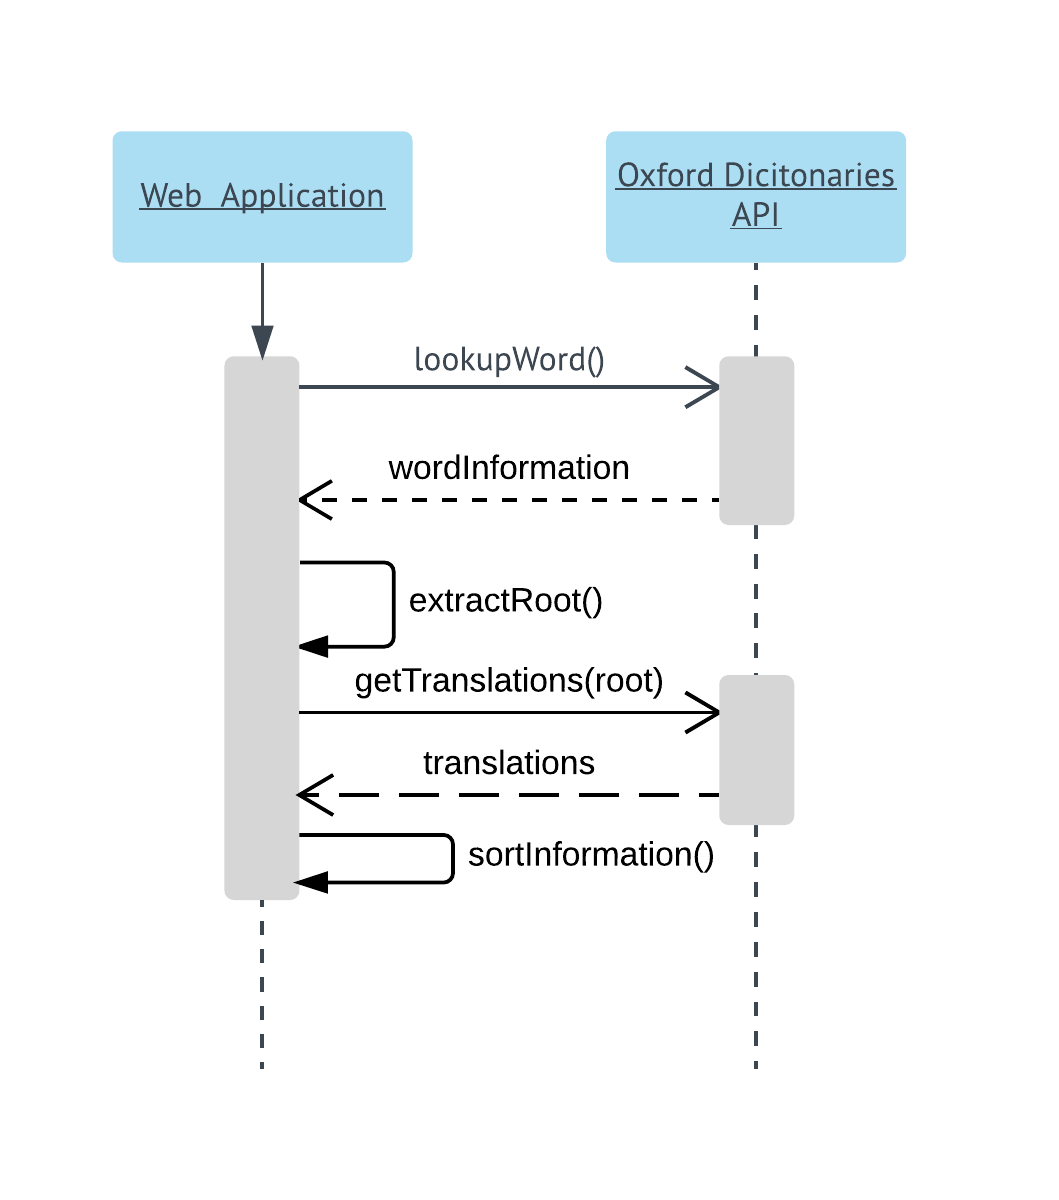
\includegraphics[width=0.7\textwidth]{Graphics/SystemsFlowOxford}
\end{center}
\end{figure}

On the first call, the root word, as provided by \textit{SpaCy}, gets its translations looked up. If one or more translation is discovered, the second call gets made, extracting the grammatical information about why the root was transformed into it's current form.

Several times throughout the grammatical feature generation and translation extraction, the results of \textit{Oxford Dictionaries API} had to be parsed in interesting ways. First of all was extracting the English translations of the words. When translations of a word are looked up using the API. It presents the results in various nested lists, first of all entries, which are all words with the same lexical category and spelling but with different meanings, then the senses or the various contexts that particular word can be used, then translation which are the valid translations of that particular word in that particular sense. As each of these are a valid translation for the word and the application has no method for distinguishing the context for that word, they should all be shown. In addition, there are exception where a word will not have any senses or a sense will not have any translations, so these have to be ignored. The code for this is in listing \ref{lst:eng}. 

\begin{lstlisting}[caption={[Translation Extraction Code] Python code for obtaining the translations of a word from the information provided by the \textit{Oxford Dictionaries API}}, label=lst:eng, breaklines=true, language=python, breakatwhitespace=true, float]
    # iterate through the uses of a word, looking for translations
    @staticmethod
    def sort_english(entries):
        en = []
        for entry in entries:
            if 'senses' in entry.keys():
                senses = entry['senses']
                for sense in senses:
                    if 'translations' in sense.keys():
                        translations = sense['translations']
                        for translation in translations:
                            en.append(translation['text'])
        return en

\end{lstlisting}


More complex was how the API presented grammatical features. All grammatical features from all possible use cases are truncated into a list, so these needed to reassembled into the use cases, an attempt was made to do this and the code for this can be seen in listing \ref{lst:gramm}.

\begin{lstlisting}[caption=Grammatical Features Extraction Code, label=lst:gramm, breaklines=true, language=python]
@staticmethod
def sort_grammar(gram_fe):
    counter = {}
    # count the occurrences of each grammatical type
    for feature in gram_fe:
        g_type = feature['type'].lower()
        if g_type in counter.keys():
            counter[g_type] += 1
        else:
            counter[g_type] = 1
    # determine the maximum
    if counter == {}:
        return []
    maximum = max(counter, key=(lambda key: counter[key]))
    # create the empty dictionaries
    sorted = [{} for _ in range(counter[maximum])]

    # create another dictionary to keep track of how many times a type has occurred while sorting.
    occurred = {}
    for key in counter.keys():
        occurred[key] = 0

    # sort the features
    for i in range(len(gram_fe)):
        g_type = gram_fe[i]['type'].lower()
        text = gram_fe[i]['text'].lower()
        o = occurred[g_type]
        sorted[o][g_type] = text
        if o == counter[g_type] - 1:
            for j in range(o, len(sorted)):
                sorted[j][g_type] = text
        occurred[g_type] += 1

    # some stuff that has to be coded manually
    if 'person' in sorted[0].keys() and 'number' in sorted[0].keys() and len(sorted) >= 2:
        if sorted[0]['person'] == 'second' and sorted[1]['person'] == 'third':
            sorted[0]['person'] = 'third'
            sorted[1]['person'] = 'second'

    if 'degree' in sorted[0].keys() and len(sorted) > 1:
        if sorted[0]['degree'] == 'positive' and sorted[1]['degree'] == 'comparative':
            sorted[0]['degree'] = 'comparative'
            sorted[1]['degree'] = 'positive'

    return sorted
\end{lstlisting}


The code starts by counting the occurrences of each type of grammatical feature, using the max to calculate the number of use cases there will be. Once it's done that, it iterates through the various features assigning the nth occurrence of each type to the nth use case. If there are more use cases than occurrences of that type of grammatical feature, the last occurrence is used for the remaining use cases. Finally, there are two sets of use use cases that were discovered to be wrong during development and therefore have code written to fix them. 

With the translations and grammatical information extracted, the information can then be given to the gloss generation code processing. 
     % Proofreading 1
\chapter{User Testing and Feedback}

Once the application had been developed, it was then user tested. For this, the application was used by German learners of various experience levels and they then gave feedback on the application. This chapter documents how the application was tested and then proceeds to analyse the feedback from the testing, examining the successes and failures of the application.

\section{Testing Methodology}

In order to carry out this testing, University of Southampton policy required that the testing had to have ethics approval from the Faculty of Physical Sciences and Engineering's ethics committee. This was applied for and approved through the ERGO system, with a submission ID number of 40080, being classed as a category C research project. While getting this approval took longer than expected, it was approved in good time. Copies of all the documents that were submitted to the ethic committee are available in the design archive. 

The plan for testing was that the user would test the application by using it to find and read three articles, they would then go on to fill out a short survey on their experiences with it. This survey asked the users the following things. 
\begin{itemize}
	\item Whether or not the application helped them understand the articles.
	
	\item Whether or not the application helped them with words in they article that they did not know.
	
	\item Whether or not the articles were of a suitable difficulty level.
	
	\item Whether or not the translations were accurate.
	
	\item Whether or not the application was easy to use.
	
	\item Whether or not the user liked the position of the gloss annotations.
	
	\item Whether or not the user would use the application if available. 
	
	\item A comment box for any additional thoughts the user may have. 
\end{itemize}


In addition, the user's use of the application was logged, so that this information could then be compared to their survey results. Doing this provided a more complete picture of the user's experience with the application, allowing for a more in-depth analysis of their results. 

\section{User Feedback and Analysis}

There were four people who tested the application. Of the four, two rated themselves beginner, one intermediate and one advanced. This was a decent range of experience levels, although more intermediate and advanced level users would have been appreciated, as this was the target demographic that the application was designed for.

\subsection{Overall Feedback for the Application}

Feedback for the application as a whole was mixed, with half the users saying that they would not use the application if it was available. One of them commented that they would prefer to use the application as a browser extension, looking up definitions for words that they discovered while browsing the web.

There was disagreement in opinion on whether or not the application was easy to use. Half of the users thought that it was, while another was neutral on the subject and the final one disagreed with the statement, presumably finding it difficult to use. This might be solvable by improving the design of the application, providing more detailed instruction on how to use the application as well as making the existence of the gloss system more obvious.


\subsection{The Article Discovery and Difficulty Rating System}

The advanced and intermediate level users said that the articles they read were of an appropriate level for them. With the advanced level one noting that they found the articles with higher difficulty ratings to be of a higher difficulty. This suggests that the level mapping system is functional in its intended use.  

A problem that occurred with one of the beginner level users, where the articles listed were mostly rated as "hard" or "very hard." This lead to a problem with the user not being able find articles of a suitable difficulty level. This problem could potentially be solved by pulling from different news sources based on the users experience level. For example, a beginner level user would get articles from sources that specifically target children or learners, while an advanced level user would get articles from a general site.

\subsection{The Gloss and Article Reader}

There was mostly positive results on whether or not the gloss helped increase the users' understanding of the articles. Mostly they thought that it had, although for some articles they thought that it had not. There is not enough data when comparing users and the articles they read to reach a conclusion as to why the gloss was not helpful in those cases. It would require multiple users reading the same article, and the nature of the testing with four users reading from different categories at different times meant that none on the users encountered any of the same articles. 

There was very mixed feedback on whether or not the application helped with understanding of unknown words. The correlation in this appears to come down to the user's experience level, with the advanced user reporting that it did not help at all, while the beginners and the intermediate ones reporting that it helped. This is probably to do with the problems faced in terms of gloss content, which are discussed in detail below.

All the users liked the position of the annotations, meaning that a marginal gloss was probably the best idea in terms of gloss position. However, one of them notes that it would be better if the annotations scrolled automatically to new ones when they appear. Expanding on this idea, it might be possible to use this as a method to dismiss the gloss items automatically as well, dismissing them when they are moved off the top of the screen.

\subsection{Gloss Content}

The most common problem found with the gloss section of the application was the fact that several words produced no usable gloss item. The words missing ranged in scope, from longer compound words that are not commonly found in dictionaries, to more common, smaller words that really should be in the dictionary. However, as this was a third party dictionary API, adding these more common words to the dictionary is not really possible. The solution is to replace the method by which translations and grammatical information are obtained. For words where translations were provided, these were considered by the users to be accurate. 

Returning to the inability for compound words to be translated, there were discussions during meetings with the project supervisor about methods that could be used  to break these words into their component parts and translate those. Adding in this functionality was dropped due to it being considered low priority, but due to the fact that the advanced and intermediate level users both attempted to gloss these words more often than the non-compound words that were in the dictionary, developing it would have most likely been beneficial for the application overall. 

In addition, a user noted several times that the content of the grammatical information provided in the gloss was wrong. The intent behind the design of the gloss was to provide every possible use case of the word in that form, but the user in question found this confusing. It would have been better to try and develop a way to determine from context the exact reason why the word was in that form, providing that as a single use case.  

Overall feedback relating to this was that the dictionary content was lacking. Future builds of the project should probably implement a better system for obtaining translations and grammatical information, as the service that was used in the current application lead overall to more incorrect grammatical information, missing translations and other mistakes than successful gloss attempts. 

A few problems relating to the design of the gloss were also found in the application. Most notably was the fact that gloss items for words over a certain length are impossible to dismiss without zooming out in the web page. Another problem that was noted by one of the users, was that the green colour of the noun glosses and the red colour of other glosses implied success and failure respectively, none of the other users commented on this but the colour scheme of the gloss is easily adjustable.


          % Proofreading 1
\chapter{Evaluation of the Project}           % Proofreading 1
\chapter{Conclusion and Possible Future Work}

This project set out to develop an application to allow German learners to more easily discover and read German language articles, the application developed in the process achieved this, as most of the users who tested it thought that it helped them. However, the bugs in application left it as a sub-par experience, with half the testers not interested in a commercial application. 

The application was designed and coded in a logical, structured way. although more advanced techniques that used machine learning algorithms were not used, they were considered during the development cycle but were not implemented due to time constraints.

Developing the application further, in the hopes of launching commercially, would probably require a restructuring  of the project into something similar to the idea that was expressed in the evaluation. The design of the gloss entries as well as application as a whole would most likely need professional input as the current design is something that was put together using various elements from pre existing CSS libraries and not really something for a professional application.

The translation software of the application should be replaced as most of the bugs in the application were caused by that, so a large amount of source code would have to be rewritten to interface the application with the new translation software.

There are various legal problems that a commercial version of the application would have to deal with, particularly the re use of the article content. A commercial application would have to make sure that the articles are licensed from their various sources as the articles, being recent, are all still in copyright.

Performing all of these actions for a commercial launch of the application would be a massive undertaking and not one worth doing at the time of writing due to financial constraints. Even if it were, the lack of intent from the testers to use the application suggests a commercial launch would likely require even more work. At some point in the future, a commercial release may be a viable option, but at that point rewriting the entire code base will probably be more feasible due to potential new technologies.            % Proofreading 1
\appendix
\chapter{Technologies Used}

\begin{description}
	\item[SpaCy] is a natural language processing python library with a publicly available German language model. 
	
	It can be found at \url{https://spacy.io/}
	
	\item[Textacy] builds on Spacy to provide higher-level natural language processing. 
	
	It can be found at \url{http://textacy.readthedocs.io/en/stable/}
	
	\item[newspaper] is a python library that can extract the plain text content from online articles. 
	
	It can be found at \url{http://newspaper.readthedocs.io/en/latest/}
	
	\item[Flask] is microframework for hosting web applications in python. 
	
	It can be found at \url{http://flask.pocoo.org/}
	
	\item[Bootstrap] is a CSS toolkit that provides a comprehensive grid system as well as some pre-built elements. 
	
	It can be found at \url{https://getbootstrap.com/}
	
	\item[JQuery] is a JavaScript library designed to make page traversal and manipulation easier.
	
	It can be found at \url{https://jquery.com/}
	
	\item[Oxford Dictionaires API] is an API designed to provide definitions, translations and conjugations for several languages. 
	
	It can be found at \url{https://developer.oxforddictionaries.com/}
	
	\item[Google News] provides articles about recent topics from a variety of sources. 
	
	It can be found at \url{https://news.google.com/news/?ned=de\&gl=DE\&hl=de}
\end{description}
\chapter{Contents of Design Archive}
\begin{description}
	\item[articles.py] Classes for the articles and the article discovery and rating system system.
	
	\item[categories.json] Category listings, in JSON format to be easily editable.
	
	\item[dictionary.py] Dictionary lookup class and a class for storing dictionary entries.
	
	\item[gloss\_app.py] Central controller of the application.
	
	\item[Pipfile] Python dependencies, install with pipenv.
	
	\item[Pipfile.lock] Python dependencies, install with pipenv.
	
	\item[static/*] Directory containing static resources, such as JavaScript and CSS files. 
		\begin{description}
			\item[dictionary.css] CSS classes for the gloss system specifically.
			
			\item[get\_translations.js] AJAX code for getting the gloss from the application server and then displaying it.
			
			\item[style.css] CSS classes for the application as a whole.
		\end{description}
	
	\item[templates/*] Display templates for the application.
		\begin{description}
			\item[article.html] Template for the article display view.
			
			\item[entry.html] Template for individual gloss entries.
			
			\item[finish.html] Template for the finished testing view.
			
			\item[home.html] Template for the category selection view.
			
			\item[main.html] Parent template for the others, except for entry.html.
			
			\item[search.html] Template for the article listing view. 
		\end{description}
	

\end{description}
\chapter{Original Project Brief}

\section{Problem}

There have been a number of e-learning tools developed to assist people with the learning of foreign languages. Very few of these tools provided real-time assistance when a person is trying to read a text and of the ones that do, very few tailor this assistance to the user's current ability with the language.

\section{Goals}

To build a tool that when given a text, such as a news article or opinion piece in German. The tool will then take the text, analyse it and then proceed to identify and highlight the words that are either unknown to the user or difficult for them to understand.

The user should then be able to click on this word and see both a translation of this word as well as any grammatical rules associated with the word, for example the root word and how the word was mutated for verbs or the gender of the word for nouns.

The tool will also be responsive, adjusting which words it highlights based on which words the user has clicked while reading previous articles.

\section{Scope}

I will be building a web application that fills the above goals. It will allow users to log on, then allow them to submit articles from German language news websites, the tool will then scan the article, and return a version of it with the words that are unknown or unfamiliar to the user highlighted and clickable.

The application will start by asking the user for their skill level on a scale of one to ten. It will then adjust  its understanding of the user's skill based on which words the user needs help with.

The German language has been chosen for this as it is a language that I am familiar enough with in order to write this tool.


\backmatter
%\bibliographystyle{ecs}
%\bibliography{Bibliography}
\printbibliography
\end{document}
%% ----------------------------------------------------------------
